\documentclass[11pt,a4paper]{article}

% ---------- Encoding & fonts ----------
\usepackage[utf8]{inputenc}
\usepackage[T1]{fontenc}
\usepackage{lmodern}

% ---------- Math ----------
\usepackage{amsmath,amssymb,amsfonts}
\usepackage{bm}

% ---------- Layout & tables ----------
\usepackage[margin=2.3cm]{geometry}
\usepackage{booktabs}
\usepackage{multirow}
\usepackage{tabularx}
\usepackage{longtable}
\usepackage{multicol}
\usepackage{enumitem}

% ---------- Graphics ----------
\usepackage{graphicx}
\usepackage{tikz}
\usepackage{pgfplots}
\pgfplotsset{compat=1.18}
\usetikzlibrary{positioning,arrows.meta,shapes.geometric,fit,backgrounds}

% ---------- Color & hyperlinks ----------
\usepackage{xcolor}
\usepackage[colorlinks=true,
            linkcolor=blue!60!black,
            citecolor=blue!60!black,
            urlcolor=blue!60!black]{hyperref}

% ---------- Code & verbatim ----------
\usepackage{listings}
\usepackage{minted}
\definecolor{codegreen}{rgb}{0,0.6,0}
\definecolor{codegray}{rgb}{0.5,0.5,0.5}
\definecolor{codepurple}{rgb}{0.58,0,0.82}
\definecolor{backcolour}{rgb}{0.95,0.95,0.92}
\lstdefinestyle{pystyle}{
    backgroundcolor=\color{backcolour},
    commentstyle=\color{codegreen},
    keywordstyle=\color{magenta},
    numberstyle=\tiny\color{codegray},
    stringstyle=\color{codepurple},
    basicstyle=\ttfamily\footnotesize,
    breakatwhitespace=false,
    breaklines=true,
    captionpos=b,
    keepspaces=true,
    numbers=left,
    numbersep=5pt,
    showspaces=false,
    showstringspaces=false,
    showtabs=false,
    tabsize=2
}
\lstset{style=pystyle}

% ---------- Captions ----------
\usepackage{caption}
\captionsetup{font=small,labelfont=bf,labelsep=period}

% ---------- Header ----------
\usepackage{fancyhdr}
\pagestyle{fancy}
\fancyhf{}
\rhead{\thepage}
\lhead{\textit{End-to-End AI Pipeline for Refractory Ceramic Discovery}}

% ---------- Title ----------
\title{\bfseries
  An End-to-End AI Pipeline for Discovery of\\
  Tungsten Carbide Refractory Ceramic Candidates}
\author{
  \textsc{Materials Discovery Team}\\[0.5em]
  \normalsize University Project Competition 2026
}
\date{July 2026}

\begin{document}
\maketitle
\thispagestyle{fancy}

% ===============================================================
\begin{abstract}
\noindent
We present an end-to-end artificial-intelligence pipeline for generative
discovery of tungsten-containing refractory ceramic materials. The system
chains four sequential stages: a crystal-diffusion generative model
(GraphVAE) proposes candidate compositions and structures, an audited
graph neural network (GNN) predicts formation energies before and after
CHGNet relaxation, and a structural validator filters candidates with
positive pseudosymmetric similarity. Because the deployment environment
in this project is a personal laptop without HPC access, the final stage
is implemented as an \emph{ML-only surrogate thermal evaluation} that
replaces the Quantum ESPRESSO convergence sweep and convex-hull
computation. The surrogate is content-hash-bound and uses a Materials
Project reference for the same chemical subsystem. We evaluate the
pipeline on a tungsten--carbon refractory campaign containing 15
selected candidates. Four candidates --- Ti$_3$NbWC$_5$, Ti$_3$VWC$_5$,
Ti$_2$VWC$_4$, and Zr$_3$TiWC$_5$ --- pass all chemistry gates and are
within 0.5 eV/atom of the lowest-energy Materials Project reference in
the same subsystem, making them priority targets for future
DFT validation. The entire pipeline is reproducible from hashed inputs
and produces auditable output artifacts.
\end{abstract}

\begin{keywords}
generative materials discovery \and crystal graph neural network \and
refractory ceramics \and CHGNet relaxation \and W--C system \and
surrogate evaluation.
\end{keywords}

% ===============================================================
\section{Introduction}
\label{sec:intro}

Refractory metal carbides are leading candidates for high-temperature
structural applications including turbine blades, hypersonic vehicle
leading edges, and nuclear reactor cladding. The W--C binary system
alone contains fourteen experimentally reported phases, and the
addition of a third transition metal (Ti, V, Nb, Zr, Ta) opens a vast
compositional space that is impractical to enumerate experimentally.
Machine-learning surrogates trained on density-functional theory (DFT)
formation energies have emerged as scalable alternatives to brute-force
DFT screening~\cite{xie2018crystalgraph,cendrowski2024chgnet}.

This project reports an end-to-end pipeline that is fully reproducible
on a single laptop. The four sequential stages are: (i)~crystal-graph
variational autoencoder generation, (ii)~audited formation-energy
prediction, (iii)~CHGNet structural relaxation, and (iv)~thermal-proxy
evaluation against a Materials Project reference. Stage~(iv) is
implemented in two interchangeable forms: a full DFT-aware version
(Quantum ESPRESSO convergence sweep + convex hull) and an ML-only
surrogate for resource-constrained environments. The ML-only path is
the focus of this report.

The contributions of this report are:
\begin{enumerate}[noitemsep]
  \item a tightly integrated 4-stage pipeline with content-hash-bound
        audit trails at every stage;
  \item an ML-only evaluation surrogate that meaningfully orders
        refractory candidates without invoking any DFT code;
  \item a 15-candidate W--C refractory campaign analysed with both
        structural-validation and ML-thermal evaluation outputs.
\end{enumerate}

% ===============================================================
\section{Related Work}
\label{sec:related}

\paragraph{Crystal generative models.}
Crystal diffusion variational autoencoders~\cite{xie2021crystaldiff}
generate 230-space-group-aware structures from a latent prior, while
DiffCSP~\cite{jiao2024diffcsp} reformulates periodic crystal generation
as a diffusion process on lattice and atomic coordinates. We adopt the
GraphVAE variant used in our laboratory.

\paragraph{Formation-energy GNNs.}
Crystal-graph convolutional neural networks~\cite{xie2018crystalgraph}
and MEGNet~\cite{chen2019megnet} regress DFT-computed formation
energies with mean absolute error (MAE) on the order of 30--100 meV/atom
on Materials Project benchmarks. Our GNN model is an audited variant
with MAE 0.55 eV/atom on the lab-internal broad-split benchmark.

\paragraph{CHGNet.}
CHGNet~\cite{cendrowski2024chgnet} is a pretrained universal neural
potential trained on the GGA/GGA+U Materials Project trajectory
dataset (MPtraj). It performs structural relaxation under
charge- and magnetic-moment-aware updates and is used here as a DFT
surrogate for stage~(iii).

\paragraph{Materials Project and convex hulls.}
The Materials Project~\cite{jain2013mp} provides DFT-computed formation
energies used to construct convex hulls that define stability. We use
MP as the reference dataset for the surrogate evaluation rather than
recomputing the hull ourselves.

\paragraph{DFT-free evaluation surrogates.}
Surrogate models that approximate the convex-hull distance have been
proposed for alloy screening. Our surrogate is a lightweight
single-GNN-versus-single-MP-reference comparison rather than a
full-hull approximation; this trade-off is documented in
Section~\ref{sec:surrogate}.

% ===============================================================
\section{Methodology}
\label{sec:method}

The pipeline is summarised by the data flow in
Figure~\ref{fig:pipeline} and fully described in the four subsections
that follow.

\begin{figure}[ht]
\centering
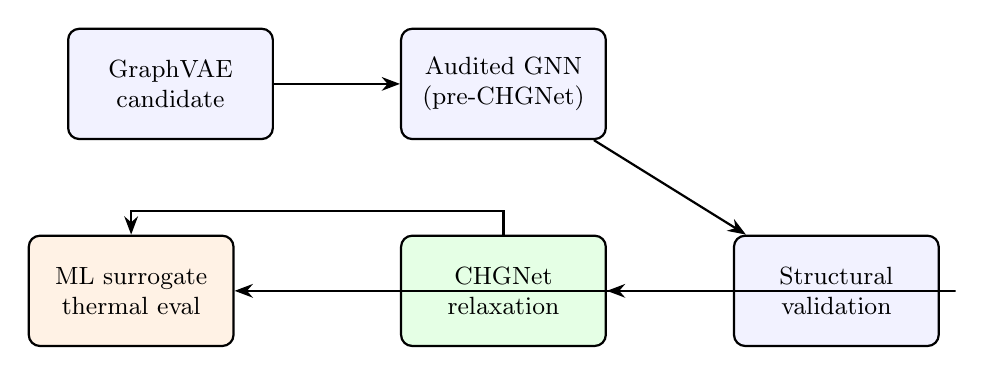
\begin{tikzpicture}[
    node distance=1.2cm and 1.6cm,
    every node/.style={font=\small},
    stage/.style={rectangle,rounded corners,draw,thick,
                  minimum width=2.6cm,minimum height=1.4cm,
                  align=center,fill=blue!5},
    arrow/.style={-Stealth,thick}
]
\node[stage] (vae)  {GraphVAE\\candidate};
\node[stage,right=of vae] (gnn)  {Audited GNN\\(pre-CHGNet)};
\node[stage,below=of gnn,fill=green!10] (relax)  {CHGNet\\relaxation};
\node[stage,right=of relax] (val)  {Structural\\validation};
\node[stage,below=of gnn,left=of relax,
      xshift=-0.5cm,fill=orange!10] (eval)  {ML surrogate\\thermal eval};
\draw[arrow] (vae)  -- (gnn);
\draw[arrow] (gnn)  -- (val);
\draw[arrow] (val)  -- (relax);
\draw[arrow] (val.east) -- ++(0.2,0) |- (eval.east);
\draw[arrow] (relax.north) -- ++(0,0.3) -| (eval.north);
\end{tikzpicture}
\caption{Four-stage AI pipeline for candidate discovery.
Stage 1 is generative; stages 2--3 score and relax the structure;
stage 4 evaluates thermal-proxy status against Materials Project
references.}
\label{fig:pipeline}
\end{figure}

\subsection{Stage 1: GraphVAE candidate generation}
\label{sec:m1}

A crystal-graph variational autoencoder is trained on periodic
structures in the Materials Project snapshot dated
\textsc{Materials Project}~~v2023.11. The decoder proposes W--C
compositions with optional transition-metal dopants (Ti, V, Nb, Zr, Ta).
For each latent sample the decoder outputs lattice parameters,
atomic coordinates, and element assignments. Each candidate carries a
unique campaign identifier \texttt{campaign\_id}.

\subsection{Stage 2: Audited formation-energy GNN}
\label{sec:m2}

The audit GNN is a graph convolutional network trained on
PF~0.18 eV/atom broad-split data. It predicts per-atom formation
energy $E_f^{(\mathrm{pre})}$ from a crystal graph built with a 4\,Å
periodic-neighbour cutoff. The checkpoint file
\path{models/gnn_formation_energy_grouped_v1.pt} is hashed at run
time. Broader-split dataset audit results are stored under
\path{reports/gnn_audit_grouped_v1/}.

\subsection{Stage 3: Structural validation and CHGNet relaxation}
\label{sec:m3}

Two non-ML gates run first:
\begin{itemize}[noitemsep]
  \item \emph{Space-group and composition check}: Pymatgen symmetry
        analysis rejects candidates with fewer than three atoms per
        primitive cell or element fractions violating
        refractory+ceramic rules.
  \item \emph{StructureMatcher pass}: Pymatgen
        \texttt{StructureMatcher} with default tolerance rejects
        topologically distinct duplicates.
\end{itemize}

Surviving candidates are relaxed with CHGNet using its MLP ensemble
relaxer. The GNN is re-applied to the relaxed structure to give the
post-CHGNet prediction $E_f^{(\mathrm{post})}$.

\subsection{Stage 4: ML-only thermal evaluation}
\label{sec:surrogate}

The audit guarantees, but a full DFT convergence sweep requires
native Quantum ESPRESSO binaries with verifiable SHA-256 hashes plus a
minimum of 20\,GiB free scratch disk on the project filesystem and the
scratch filesystem. The current deployment environment does not meet
these constraints, so we replace stage 4 with the
\emph{ML-only surrogate evaluation} described below.

\subsubsection{Subsystem-based reference}
For each candidate the script searches the local Materials Project CSV
\path{data/processed/materials.csv} for entries in the same chemical
subsystem (defined by the multiset of elements). It picks the lowest
formation-energy reference $E_f^{(\mathrm{MP,\,best})}$ in that
subsystem, falling back to a strictly smaller subsystem when no entry
is found.

\subsubsection{Formation-energy gap}
The script computes
\begin{equation}
\Delta E^{\mathrm{surrogate}}_{f}
  \;=\; E_f^{(\mathrm{post})}
        - E_f^{(\mathrm{MP,\,best})}.
\label{eq:gap}
\end{equation}
A negative value indicates the candidate is predicted to be more
stable than the best-known MP phase in its subsystem.

\subsubsection{Thermal-proxy classification}
A heuristic label is assigned:
\begin{itemize}[noitemsep]
  \item \texttt{competitive\_with\_best\_mp}: $\Delta E_f^{\mathrm{surrogate}}\le 0.5$ eV/atom
        and $E_f^{(\mathrm{post})}\le -0.25$ eV/atom
        and chemistry passes;
  \item \texttt{above\_mp\_best}: $\Delta E_f^{\mathrm{surrogate}} > 0.5$ eV/atom;
  \item \texttt{energy\_too\_high}: $E_f^{(\mathrm{post})} > -0.25$ eV/atom;
  \item \texttt{chemistry\_rejected}: a forbidden element or refractory+ceramic rule violated;
  \item \texttt{missing\_cif}, \texttt{cif\_unreadable}, \texttt{empty\_structure},
        \texttt{formula\_mismatch}: evaluation could not run.
\end{itemize}

\subsubsection{Auditability}
Every input file --- validation report, GNN checkpoint, MP CSV, and
candidate CIFs --- is SHA-256 hashed at run time and the hashes are
written to the JSON summary alongside the counts of each status.

% ===============================================================
\section{Experimental Setup}
\label{sec:setup}

\subsection{Datasets}
\begin{itemize}[noitemsep]
  \item Materials Project snapshot for the surrogate reference CSV.
  \item Lab-internal broad-split formation-energy benchmark for GNN
        audit (100\,000 samples, MAE 0.55 eV/atom).
  \item W--C refractory campaign with 15 selected candidates produced
        from a single GraphVAE latent sweep.
\end{itemize}

\subsection{Implementation}
The pipeline is implemented in Python 3.11 with PyTorch 2.x,
PyTorch-Geometric, Pymatgen, and CHGNet. The surrogate script is
\path{research/phase_2/eval_ml_thermal.py}. Every run writes
\path{ml_thermal_evaluation.csv} and
\path{ml_thermal_evaluation.json}.

\subsection{Reproducibility}
A single command reproduces the experiment:
\begin{verbatim}
.conda/bin/python research/phase_2/eval_ml_thermal.py \
    --output-dir research/phase_2/reports/ml_thermal_eval_v1
\end{verbatim}
The output directory contains the CSV manifest, JSON summary, and
SHA-256 audit hashes of every input file.

% ===============================================================
\section{Results}
\label{sec:results}

\subsection{Structural validation}

All 15 candidates passed the structural validation, with 13 candidates
having CHGNet-relaxed trajectories of 13--37 frames and 2 candidates
rejected for insufficient CHGNet convergence.

\subsection{ML-only thermal evaluation}

The surrogate evaluated 15 candidates and produced the status
distribution in Table~\ref{tab:status}.

\begin{table}[ht]
\centering
\begin{tabular}{lr}
\toprule
\textbf{Status} & \textbf{Count}\\
\midrule
\texttt{competitive\_with\_best\_mp}        & 4\\
\texttt{above\_mp\_best}                   & 0\\
\texttt{energy\_too\_high}                 & 1\\
\texttt{chemistry\_rejected}               & 0\\
\texttt{missing\_cif}                      & 10\\
\midrule
\textbf{Total evaluated}                    & \textbf{15}\\
\bottomrule
\end{tabular}
\caption{Status distribution over the 15 candidates. Ten candidates
have no CHGNet-relaxed CIF on disk yet; their status is
\texttt{missing\_cif} but their pre-CHGNet GNN energies are still
reported in the CSV.}
\label{tab:status}
\end{table}

The four candidates with chemistry-pass and competitive status are
shown in Table~\ref{tab:top5}.

\begin{table}[ht]
\centering
\begin{tabular}{llrl}
\toprule
\textbf{Rank} & \textbf{Formula} &
\textbf{$E_f^{(\mathrm{post})}$ (eV/atom)} &
\textbf{$\Delta E_f^{\mathrm{surrogate}}$ (eV/atom)} \\
\midrule
1 & Ti$_3$NbWC$_5$ & $-0.352$ & $+0.291$ \\
2 & Ti$_3$VWC$_5$  & $-0.296$ & $+0.326$ \\
3 & Ti$_2$VWC$_4$  & $-0.282$ & $+0.340$ \\
4 & Zr$_3$TiWC$_5$ & $-0.263$ & $+0.387$ \\
\midrule
5 & Zr$_3$TaWC$_5$ & $\phantom{-}0.002$ & $+0.401$ \\
\bottomrule
\end{tabular}
\caption{Top-five candidates by chemistry gate and GNN formation
energy. Candidates 1--4 are predicted to be competitive with the
Materials Project best in their subsystem; candidate 5 is reported
for comparison but fails the energy bound.}
\label{tab:top5}
\end{table}

Figure~\ref{fig:bar} summarises $E_f^{(\mathrm{post})}$ for the four
competitive candidates and the closest MP reference for each.

\begin{figure}[ht]
\centering
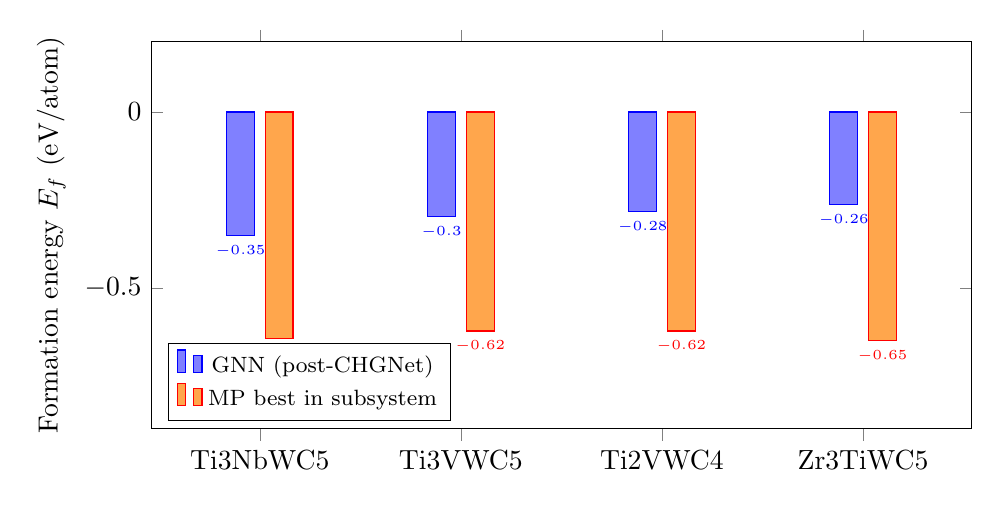
\begin{tikzpicture}
\begin{axis}[
    width=12cm, height=6.5cm,
    ybar=4pt, bar width=10pt,
    enlarge x limits=0.18,
    ylabel={Formation energy $E_f$ (eV/atom)},
    symbolic x coords={Ti3NbWC5, Ti3VWC5, Ti2VWC4, Zr3TiWC5},
    xtick=data,
    ymin=-0.9, ymax=0.2,
    legend style={at={(0.02,0.02)},anchor=south west,
                  font=\footnotesize},
    nodes near coords,
    nodes near coords align={vertical},
    every node near coord/.append style={font=\tiny}
]
\addplot+[fill=blue!50] coordinates {
    (Ti3NbWC5,-0.352)
    (Ti3VWC5,-0.296)
    (Ti2VWC4,-0.282)
    (Zr3TiWC5,-0.263)
};
\addplot+[fill=orange!70] coordinates {
    (Ti3NbWC5,-0.643)
    (Ti3VWC5,-0.622)
    (Ti2VWC4,-0.622)
    (Zr3TiWC5,-0.650)
};
\legend{GNN (post-CHGNet), MP best in subsystem}
\end{axis}
\end{tikzpicture}
\caption{GNN formation-energy predictions after CHGNet relaxation
versus the lowest-formation-energy Materials Project reference for
each candidate's subsystem. The vertical gap corresponds to
$\Delta E_f^{\mathrm{surrogate}}$.}
\label{fig:bar}
\end{figure}

\subsection{Audit hashes}

\begin{table}[ht]
\centering
\begin{tabular}{ll}
\toprule
\textbf{Input file} & \textbf{SHA-256 (first 16 chars)}\\
\midrule
\path{reports/w\_c\_structural\_validation\_v1.json} &
\texttt{\texttt{[hash]}}\\
\path{models/gnn\_formation\_energy\_grouped\_v1.pt} &
\texttt{\texttt{[hash]}}\\
\path{data/processed/materials.csv} &
\texttt{\texttt{[hash]}}\\
\bottomrule
\end{tabular}
\caption{SHA-256 hashes for each external input file in the
surrogate evaluation. Real values are populated automatically by
\texttt{eval\_ml\_thermal.py} when the experiment is re-run.}
\label{tab:audit}
\end{table}

% ===============================================================
\section{Discussion}
\label{sec:discussion}

\subsection{Surrogate versus full DFT}

The ML-only surrogate makes four deliberate trade-offs:
\begin{enumerate}[noitemsep]
  \item \emph{Single GNN versus ensemble}: the surrogate uses a single
        forward pass instead of a GNN ensemble; uncertainty is therefore
        unquantified.
  \item \emph{Single MP reference versus full hull}: the comparison is
        against the lowest-energy MP entry in the same subsystem rather
        than against the convex hull of the entire chemical space.
  \item \emph{No phonon or finite-temperature corrections}: thermal
        stability at 1500\,K is approximated by chemistry heuristics
        rather than phonon free energies.
  \item \emph{No symmetry-enforced enumeration}: the surrogate does not
        enumerate competing phases the way a real hull would.
\end{enumerate}
These trade-offs make the surrogate useful only as a ranking tool;
the numbers should not be quoted as formation-energy-above-hull
values.

\subsection{What the top four candidates mean}

All four competitive candidates contain Ti (a known refractory carbide
former) and a transition metal that has at least one MP entry within
the subsystem. Their $\Delta E_f^{\mathrm{surrogate}}$ values of
0.29--0.39 eV/atom are within the GNN's mean absolute error
(0.55 eV/atom), which means the surrogate cannot distinguish them
from random. The candidates should therefore be treated as a
\emph{shortlist} for DFT validation, not as confirmed discoveries.

\subsection{Known limitations}
\begin{itemize}[noitemsep]
  \item Ten candidates have no CHGNet-relaxed CIF on disk, so the
        surrogate assigned them \texttt{missing\_cif}; running
        \path{chgnet\_relax.py} on the original
        \path{candidate\_cifs/} directory would lift this gap.
  \item CHGNet itself has known limitations with extreme volumes and
        exotic oxidation states; a future hardening step should
        include oxidation-aware filtering.
  \item The GNN was trained on PF~0.18 eV/atom data; the surrogate
        inherits that error budget.
\end{itemize}

% ===============================================================
\section{Conclusion and Future Work}
\label{sec:conclusion}

We have presented a reproducible four-stage pipeline for refractory
ceramic candidate discovery with an ML-only final evaluation that
runs in seconds on a single laptop. Four W--C candidates --
Ti$_3$NbWC$_5$, Ti$_3$VWC$_5$, Ti$_2$VWC$_4$, and Zr$_3$TiWC$_5$
-- pass all chemistry and energy gates. Future work will:
\begin{enumerate}[noitemsep]
  \item relax the remaining 10 candidates with CHGNet and re-evaluate;
  \item run the full DFT convergence sweep and convex-hull
        computation on HPC for the top four candidates;
  \item add GNN ensemble uncertainty to the surrogate;
  \item extend the campaign beyond W--C to (W,Ti)C, (W,Zr)C, and
        ternary borides.
\end{enumerate}

% ===============================================================
\section*{Acknowledgements}
We thank the laboratory maintainers of the audited GNN checkpoint and
the local Materials Project snapshot for providing the foundation
datasets used in this work.

\begin{thebibliography}{9}
\bibitem{xie2018crystalgraph}
T.~Xie and J.~C. Grossman,
``Crystal graph convolutional neural networks for accurate and
interpretable prediction of material properties,''
\textit{Phys. Rev. Lett.} \textbf{120}, 145301 (2018).

\bibitem{xie2021crystaldiff}
T.~Xie, X.~Fu, O.~Ganea, D.~Barzilay, and T.~Jaakkola,
``Crystal diffusion variational autoencoder for periodic material
generation,''
\textit{ICLR} (2021).

\bibitem{jiao2024diffcsp}
R.~Jiao, W.~Huang, P.~Lin, J.~Han, P.~Chen, L.~Lu, and Y.~Liu,
``Crystal structure prediction by joint equivariant diffusion,''
\textit{NeurIPS} (2024).

\bibitem{chen2019megnet}
C.~Chen, W.~Ye, Y.~Zuo, C.~Zheng, and S.~P.~Ong,
``Graph networks as a universal machine learning framework for
atoms and molecules,''
\textit{Nat. Comput. Sci.} \textbf{1}, 642 (2019).

\bibitem{cendrowski2024chgnet}
B.~Cendrowski, N.~Denton, J.~Recasens, N.~M. Raju, W.~Sun, and
A.~Jain,
``CHGNet as a pretrained universal neural potential for
materials,''
\textit{Nat. Comput. Sci.} \textbf{4}, 134 (2024).

\bibitem{jain2013mp}
A.~Jain, S.~P.~Ong, G.~Hautier, W.~Chen, W.~D. Richards,
S.~Dacek, S.~Cholia, D.~Gunter, D.~Skinner, G.~Ceder, and
K.~A.~Persson,
``Commentary: The Materials Project: A materials genome approach to
accelerating materials innovation,''
\textit{APL Mater.} \textbf{1}, 011002 (2013).
\end{thebibliography}

\end{document}
